%%%%%%% By Michał Swoboda
%%%%%%% Poprawki by Błażej Kowalczyk
%%%%%%% Uporządkował pewne rzeczy Bartłomiej Kurosz

\documentclass[xcolor=dvipsnames]{beamer}%[hyperref={pdfpagelabels=false}]{beamer}
\usepackage{lmodern}
\usepackage{polski}
\usepackage[utf8]{inputenc}
\usepackage{amsfonts}
\usepackage{tikz}

%%%%%%%%%%%%%%%% Początek poleceń własnych
% Maksymalna dostępna wysokość pola w~prezentacji (między wąskim nagłówkiem a~stopką)
% dobrana eksperymentalnie - może w~przyszłości po prostu ją wyliczać???
\newlength{\maxheight}
\setlength{\maxheight}{\paperheight}
\addtolength{\maxheight}{-17.85pt}  % tyle zajmuje naczółek ze stopką 

% Polecenie do dokładania wycentrowanych rzeczy (zdjęć) na środku slajdu 
% bez tytulariów (ale ze stopką i~naczółkiem)
% By uzyskać obrazek "na całą stronę" jako argumentu należy użyć
% 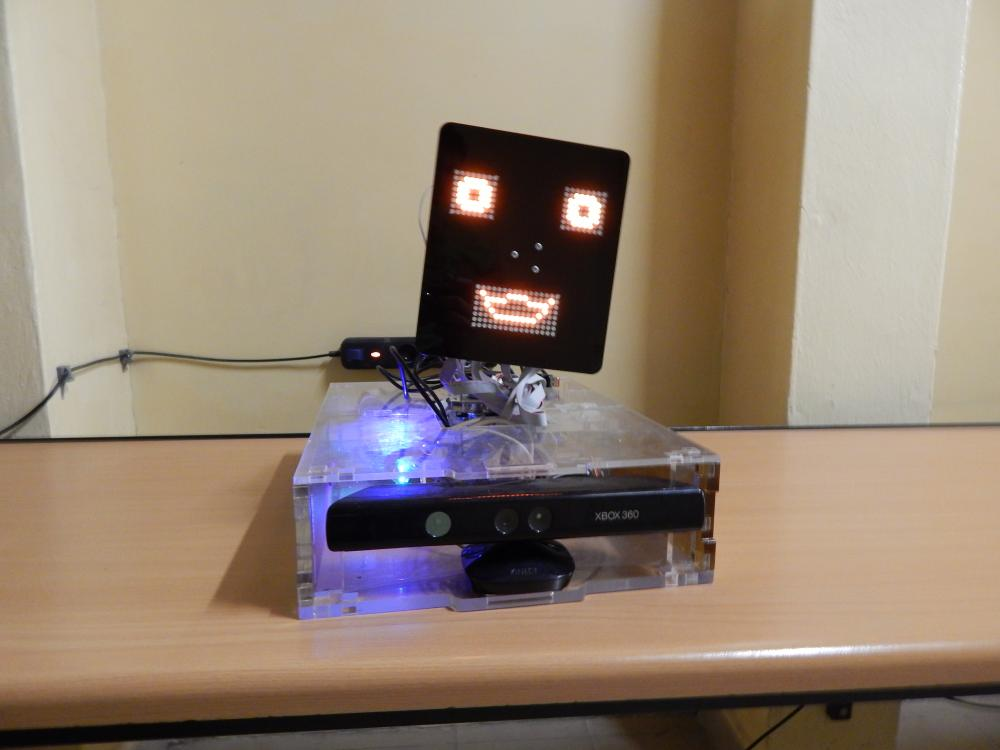
\includegraphics[height=\maxheight,width=\paperwidth]{figure/balbina.jpg}
% Jeśli nie chcesz zmian proporcji - zrezygnuj z~jednego z~wymiarów
% Obrazki za duże przykryją naczółek strony
% By wszystko było na swoim miejscu potrzebna jest dwukrotna kompilacja 
\newcommand{\framecentered}[1]{
  \setbeamertemplate{background canvas}{}
  \begin{frame}[c]
    \begin{tikzpicture}[overlay, remember picture]
      \node[anchor=center] at (current page.center) 
      {#1};
    \end{tikzpicture}
  \end{frame}}
%%%%%%%%%%%%%%%% Koniec poleceń własnych

%%%%%%%%%%%%%%%%Początek ustawień
\usebackgroundtemplate{%
  
\includegraphics[width=\paperwidth,height=\paperheight]{background/tlo.pdf}} 

\usepackage{beamerthemesplit}
\useoutertheme{infolines}
\useinnertheme{rounded}

\definecolor{konar2}{RGB}{240,152,52}
\definecolor{konar}{RGB}{151,58,66}

\setbeamercolor{block title}{fg=black,bg=konar2}
\setbeamercolor{block title alerted}{fg=konar2,bg=black}

\setbeamertemplate{navigation symbols}{}
\setbeamercolor{frametitle}{fg=white,bg=konar}
\setbeamercolor{section in head/foot}{bg=konar}
\setbeamercolor{author in head/foot}{fg=Black,bg=konar2}
\setbeamercolor{date in head/foot}{fg=Black}
\setbeamercolor{title in head/foot}{fg=white, bg=konar}
\setbeamercolor{section in head/foot}{fg=white}
\setbeamercolor{titlelike}{fg=black}
\setbeamercolor{structure}{bg=black, fg=konar2}
\setbeamercolor{subsection in head/foot}{fg=black}
\setbeamercolor{item}{bg=white}

%%%%%%%%%%%%%%%%%Koniec Ustawień

%%%%%%%%%%%%%%%%% SLAJD TYTUŁOWY

\title[Skrócony Wzór]{Wzór prezentacji na tle KoNaRowym } %tytuł prezentacji, skrócony w razie za długiej nazwy nie mieszczącej się w stopce
\author[Skrócony Autor]{Michał Swoboda} %autor, skrócony autor w razie za długiej nazwy nie mieszczącej się w stopce
\date{\today}  %data

%%%%%%%%%%%%%%%%%



\begin{document}

\begin{frame}
\titlepage
\end{frame} 

\begin{frame}
\frametitle{Plan prezentacji}
\tableofcontents
\end{frame}

\section{Wstęp}
\subsection{Pierwszy merytoryczny slajd}
\begin{frame} %początek sladjdu
\frametitle{Nazwa Slajdu}
\framesubtitle{Podnazwa slajdu} %Opcjonalnie

\centering Zawartość tekstowa
		
\end{frame}%koniec slajdu

\subsection{Drugi merytoryczny slajd}
\begin{frame}
\frametitle{Pojawianie się puntków}
\framesubtitle{Bardzo efektowne}
	\begin{itemize}
		\item Pierwszy punkt
		\pause
		\item Drugi punkt
		\pause
		\item Trzeci punkt
	\end{itemize}
\end{frame}

\section{Koniec}
\subsection{Wstawianie Rysunku}
\begin{frame}
	\frametitle{Przepiękna i zjawiskowa}
	\centering \begin{figure}
   		       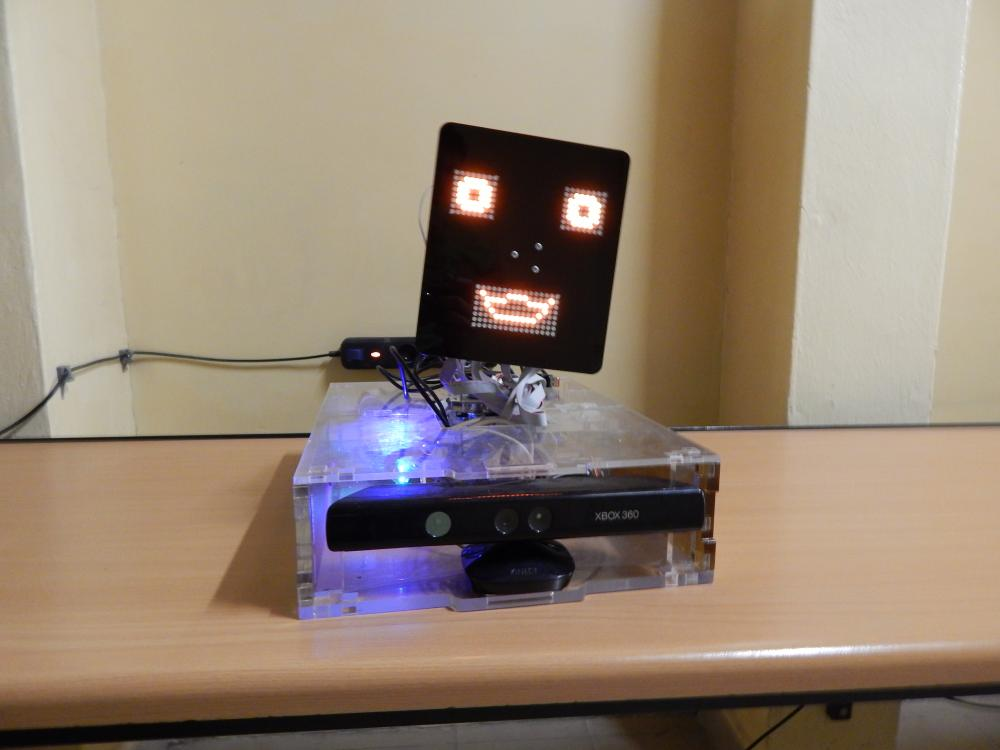
\includegraphics[height=5cm]{figure/balbina.jpg}
		       \caption{Balbina}
		       \end{figure}
\end{frame}

% Balbina średnia bez tytulariów
\framecentered{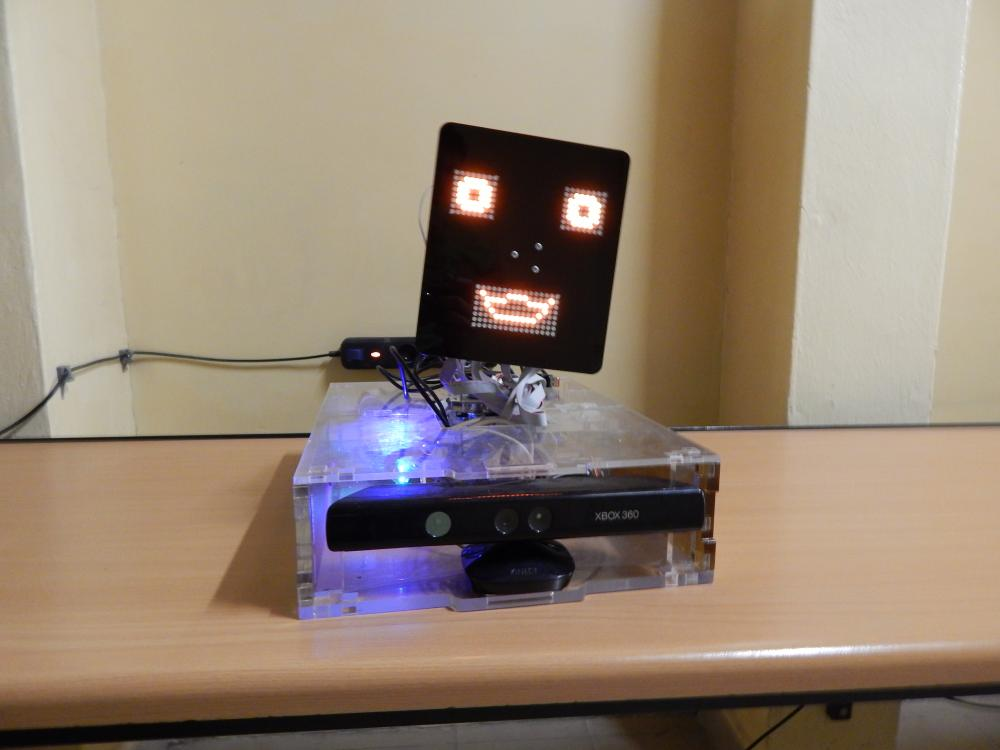
\includegraphics[width=0.7\paperwidth]{figure/balbina.jpg}}
% Balbina porozciągana ale na całość
\framecentered{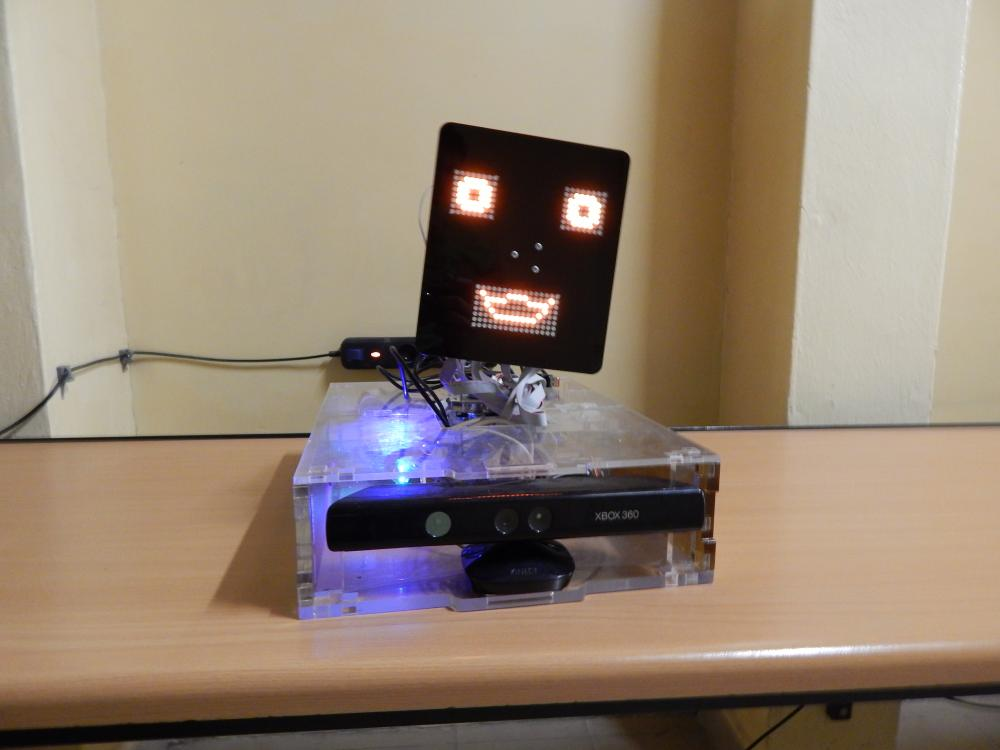
\includegraphics[height=\maxheight,width=\paperwidth]{figure/balbina.jpg}}
% Balbina dopasowana na wysokość
\framecentered{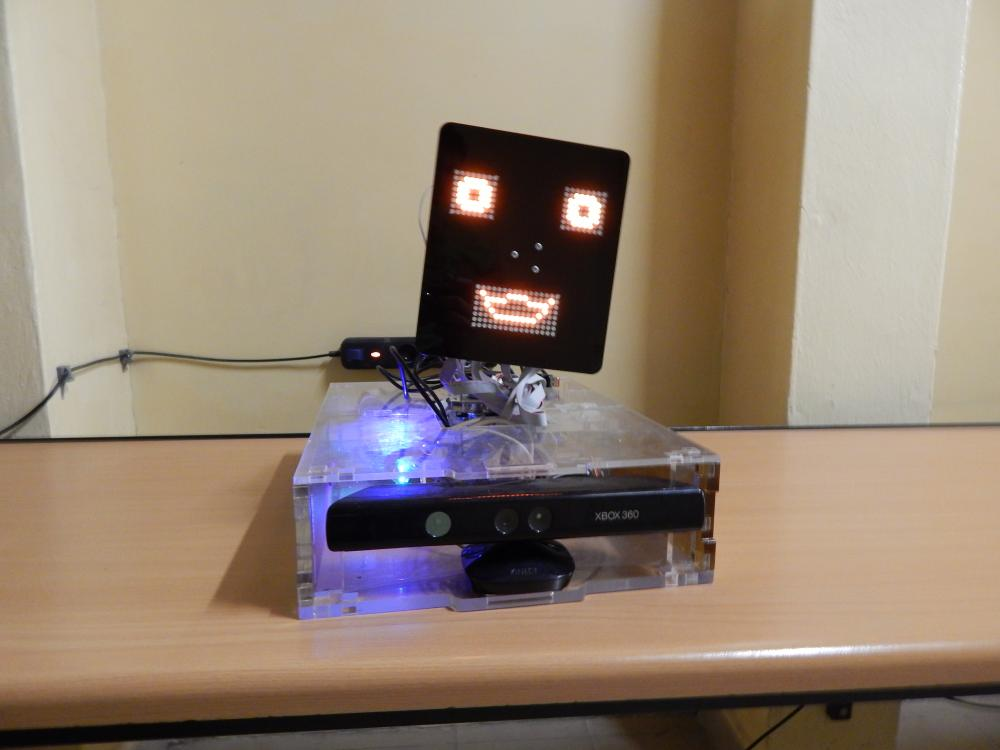
\includegraphics[height=\maxheight]{figure/balbina.jpg}}
% Balbina za duża - zakrywa naczółek
\framecentered{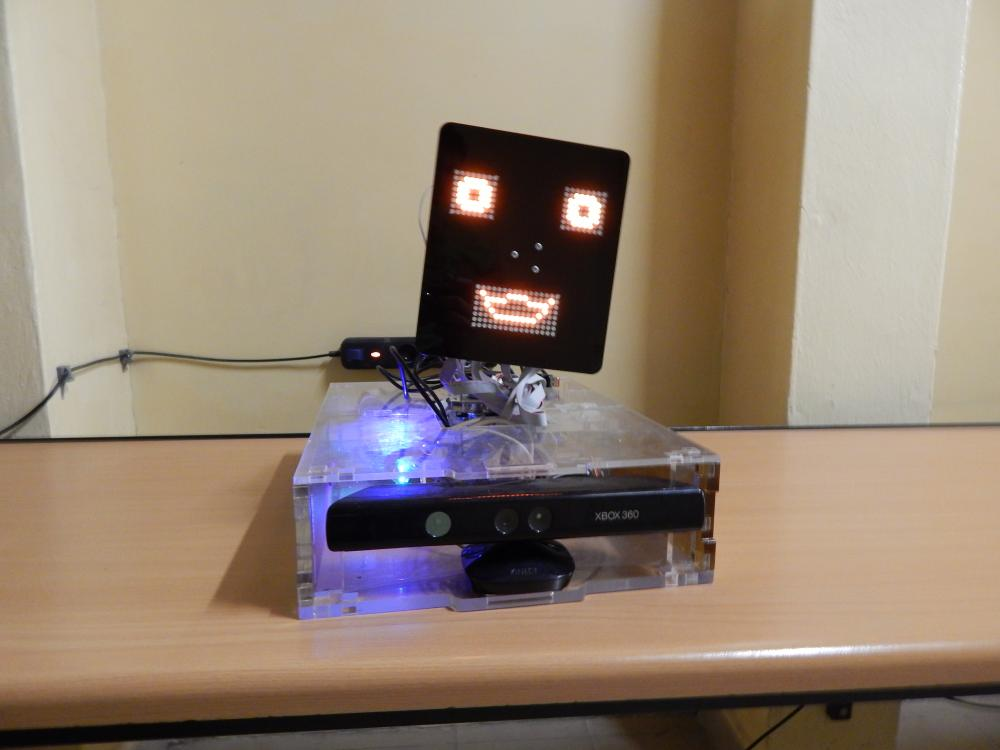
\includegraphics[width=\paperwidth]{figure/balbina.jpg}}

\subsection{Problemy}
\begin{frame}
\frametitle{Pomocy?}
	\begin{block}{Gdzie szukać porad}
	Pomocy szukajcie w internecie, to nie jest takie trudne : )
	\end{block}
\end{frame}
	
	

\end{document}